\newpage

\section{Návrh aplikácie}

V tejto kapitole sa budeme zaoberať zvolenými technológiamy a abstraktným návrhom 
aplikácie.

\subsection{Platforma}

Prácu som sa rozhodol vypracovať vo forme webovej aplikácie.
Túto formu som zvolili najmä pre väčšiu dostupnosť pre koncového používateľa.
Tak isto veľkým plus je že celá aplikácie beží na strane tvorcu takže prípadne zmeny 
v systéme nebude potrebne synchronizovať naprieč viacerímy zariadeniamy. 
Ďaľšou výhodou je redukovanie problémov zo synchronizáciou databáza medzi koncovímy
zariadeniamy.

Tak isto protabilita riešenia je pomerne dobrá, nepotrebujem sa zaoberať rôznymi verziamy
operačných systémov. Proti tomuto by sa dalo argumentovať rozdielmy medzi 
internetovými prehliadačmy a potrebu responzívneho dizajnu pre mobilné zariadenia,
ale toto všetko sa dá jednoducho vyriešiť voľbou správny grafických knižníc.

Keďže sa jedná o webovú aplikáciu, bude bežať čiastočne vo forme klient serve ako 
html, css a javascript kód bežiaci vo vyhľadávači používateľa a php kód bežiaci na strane.

\paragraph{Klient}

Klientska časť je postavená na JavaScripte, HTML a CSS3. Aby som zabezpečil responzívny 
dyzajn a portabilitu naprieč prehliadačmy, rozhodol som sa použiť knižnicu
Bootstrap\footnote{http://getbootstrap.com/},
ktorá ja postavená na CSS3 a jQuery. Vďaka nej nemusím kontrolovať vyzualnu stránku v 
rôznych prehliadačoch a vytvorenie dizajnu, ktorý dobre spolupracuje z rôznimy rozmermy
obrazoviek a rozlíšení, ma stojí pomerne málo námahy. Tak isto plánujem použiť 
jQuery\footnote{https://jquery.com/} v prípade potreby implementácie logiky na klientskej strane
a CSS3\footnote{http://www.css3.info/} v prípade potreby hlbších zásahov do grafiky.

\paragraph{Server}

Na strane servera som sa rozhodol použiť jazyk PHP5\footnote{http://php.net/}
najmä z dôvodu že s ním mám predošlé 
skúsenosti, tak isto pre tento jazyk sa dá ľahko vyhladať hosting a má veľmi rozsiahlu 
dokumentáciu. Avšak v tomto jazyku je nedostatok štruktúri čo niekedy môže viesť k veľkým
neudržateľným aplikáciam, preto som sa rozhodol použiť aplikačný rámec (angl. framework) 
Yii2\footnote{http://www.yiiframework.com/} ktorý má sadú odporúčaných praktík vďaka
ktorím je aplikácia dlhodobo udržateľná.
Ďaľšou výhodou je že tento aplikačný rámec má v sebe zapracované všetky hore uvedené
klientské knižnice, čím uľahčuje prácu s nimy.
Tak isto nám tento aplikačný rámec umožňuje používať rôzne databázy vďaka svojmu modulu 
DAO\footnote{https://github.com/yiisoft/yii2/blob/master/docs/guide/db-dao.md}
pomocou ktorý modeluje SQL dotazy. Avšak niektoré zložitejšie dotazy sa v ňom nedajú
namodelovať. Ako databázu som zvolil MySQL\footnote{https://www.mysql.com/}
vďaka jej rýchlosti, popularite ale najmä dostupnosti.

\paragraph{Vývojová platforma}

Ako správcu verzí som sa rozhodol použiť git\footnote{http://git-scm.com/}.
Tento nástroj je pomerne jednoduchý na 
ovládanie a spoľahlivý. Tak isto existuje množstvo internetových služieb kde sa pomocov
neho dá zálohovať. Verziovanie dopĺňam správou balíkov pomocov manažéra balíkov 
Composer\footnote{https://getcomposer.org/}

Na testovanie som sa rozhodol použíť na PHPUnit postavený Codeception, ktorý 
je integrovaný do Yii2.

Ako editor používam Vim z množstvom prídavných modulov.

\subsection{Základné rozvrhnutie aplikácie}

Keďže ide o webovskú aplikáciu, na najvyššej úrovni bude postavená na vzore 
Klient-Server. Avšak z dôvodu bezpečnosti sa bude väčšina úloh vykonávať na servery.
Aplikácia bude získavať dáta z už existujúce databázy
hudobných dokumentov\footnote{http://www.supermusic.sk/}.
Tieto dáta chcem doplniť o socialne tagy zo služby
last.fm\footnote{http://www.last.fm/home}.
Nad týmito dátamy sa bude vykonávať vyhľadávanie, ale najmä 
odporúčanie. Základný náčrt aplikácie môžeme vydieť na 
obrázku \ref{fig:app_structure}.


\begin{figure}
    \begin{center}
        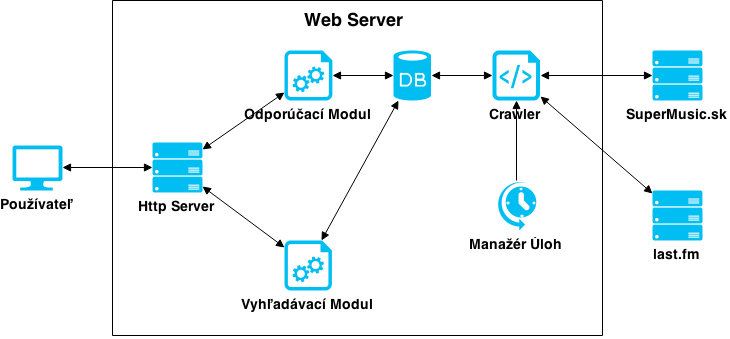
\includegraphics[scale=0.55]{app_structure}
        \caption{Štruktúra aplikácie}
        \label{fig:app_structure}
    \end{center}
\end{figure}

Aplikácia sa bude skladať z dôch hlavný oddelených subsystémov

\begin{itemize}
\item{odporúčanie (spúšťané používateľom cez prehliadač),}
\item{indexovanie dokumentov (séria úloh spúšťaná manažérom úloh).}
\end{itemize}

\subsection{Špecifikácia služieb}

Aplikácia by mala poskytovať niekoľko základných služieb

\begin{itemize}
\item{vyhľadávanie dokumentov,}
\item{najdenie podobných dokumentov aktuálne zobrazenému dokumentu,}
\item{odporúčanie dokumentov,}
\item{zostavenie spevníka.}
\end{itemize}

Prvé dve funkcionality sú vytvorené najmä z dôvodu že v danej doméne 
sa ťažko získavajú preferencie, ich jedinou úlohou je získanie základných
preferencií používateľa na základe ktorých budeme vytvárať odporúčania.

Pre zabezpečenie týchto funkcií bude potrebované udržiavať databázu dokumentov
ktorá sa bude pravidelne aktualizovať. Toto bude zabepečovať Kravler (angl. crawler)
ktorý bude vykonávať činnosti

\begin{itemize}
\item{prehľadávanie supermusic po nových dokuemntoch,}
\item{prehľadávanie supermusic po nových interprétoch,}
\item{sťahovanie dokumentov zo supermusic,}
\item{sťahovanie značiek z last.fm,}
\item{váhovanie značiek.}
\end{itemize}

Kravler bude implementovaný ako aplikácia pre príkazový riadok
aby sa dal použiť z manažérom úloh.

\paragraph{Odporúčanie}

Na odporúčanie by som chcel využiť filtrovanie na základe obsahu
spolú z vlastným algoritmom na určenie dlhodobých, krátkodobých a
sezonných záujmov.

\section{Implementácia}

\subsection{Datový model}

\paragraph{Model dokumentu}

Dokument bude reprezentovaný svojím názvom, typom a značkamy,
pričom zančky budú mať doménu na základe toho či vznikli
z názvu dokumentu, jeho typu, názvu interpréta alebo alebo
boli získane zo služby last.fm.

Čiže dokument bude uložený v trojrozmernom vektorovom priestore,
kde prvá súradnica budú dokumenty \(D = {d_1, d_2,... d_n}\),
ďaľšia súradnica budú značky \(Z = {z_1, z_2,.. z_n}\) a posledná 
súradnica budú domény \(D = {d_{názov}, d_{interpret}, d_{typ}, d_{tag}}\).

\paragraph{Model používateľa}

Používateľov profil bude reprezentovaný históriou navštívených značiek.
Bude sa ukladať pre každú navštívenu značku a jeden riadok bude obsahovať 
informácie \(row = {d_i, u_j, z_l, čas}\) kde \(d_i\) je zobrazený dokument,
\(u_j\) je používateľ ktorý dokument zobrazil, \(z_l\) je značka ktorá bola zobrazená.

Celú túto schému môžeme vydieť na obrázku \ref{fig:user_document_data_model}.


\begin{figure}
    \begin{center}
        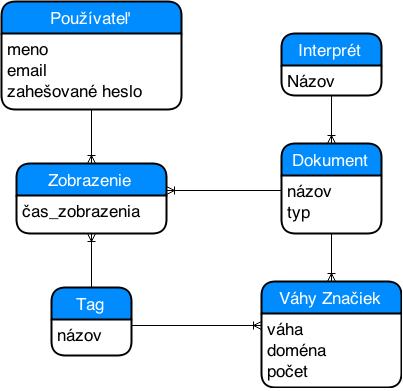
\includegraphics[scale=0.55]{user_document_data_model}
        \caption{Zjednodušený datový model}
        \label{fig:user_document_data_model}
    \end{center}
\end{figure}

\subsection{Indexovanie dokumentov a váhovanie}

\paragraph{Kravler}

Kravler (angl. crawler) je program slúžiacy na prehľadávanie webu za účelom
indexovania\footnote{http://en.wikipedia.org/wiki/Web\_crawler}. Kravler vykonáva niekoľko
operácií v rámci aplikácie, je implementovaný ako jednoduchý program príkazového riadku.
Každá z jeho operáci sa v prípade potreby dá vykonať osobytne. Toto je hlavne potrebné ak by
sa zmenili parametre indexovania. Na obrázku \ref{fig:crawler_flowchart} môžeme vydieť digram
akcií kravleru.

\begin{figure}
    \begin{center}
        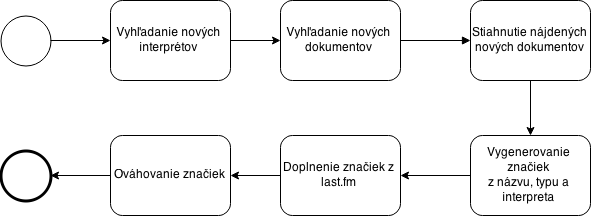
\includegraphics[scale=0.55]{crawler_flowchart}
        \caption{BPMN Digram kravleru}
        \label{fig:crawler_flowchart}
    \end{center}
\end{figure}

\paragraph{Vyhľadanie nových interpretov}

\paragraph{Vyhľadanie nových dokumentov}

Pri tejto akcií sa využíva spôsob triedenie piesni na supermusic. Piesne sú triedené podľa
abecedy a na ich zobrazenie slúži adresa \uv{http://www.supermusic.sk/piesne.php?od=\$param}.
pričom param je reťazec na ktorý majú piesne začínať. Experimentálne som overil že 
na zobrazenie skoro všetkých dokumentov mi stačí použiť dva znaky.

Prvý znak je anglická abeceda rozšírená o niekoľko slovenský a českých interpunkčný písmen
plus hviezda. Teda v provom rade sú písmená z množiny \({A, B, C, D, E, F, G, H, I, J, K, L, M,
N, O, P, Q, R, S, T, U, V, X, Y, Z, Č. Ď, Ľ, Ř, Š, Ť, Ž, *}\),
v druhej rade už je anglická abeceda.

Následne sa snaží získať zoznam piesni zo staihnutej stránky, za týmto účelom používam try
XPath výrazy

\begin{itemize}
\item{\uv{//table[@width=740]//td/a/text()} na vyhľadanie všetkých názvou piesni,}
\item{\uv{//table[@width=740]//td/a/@href} na ziskanie univerzánlneho identifikátora piesne,}
\item{\uv{//table[@width=740]//td/imt/@src} na získanie typu dokumentu,}
\item{\uv{//table[@width=740]//td/text()} na získanie názvu interpréta.}
\end{itemize}

Tieto parametre sa následne ďalej spracuvávaju.

\paragraph{Stiahnutie nových dokumentov}

\paragraph{Vygenerovanie značiek}

\paragraph{Doplnenie značiek z last.fm}

\paragraph{Váhovanie značiek dokumentov}

Tento model sa v MySQL nazýva model prírodzeného jazyka (angl. Natural Language Model),
ktorý porovnáva vlastnosti dokumentov na základe abstrakcie priestoru,
v ktorom sú jednou dimenziou vlastnosti jedného dokuemntu a druhou vlastností druhého
dokumentu, prípade vyhľadávacieho reťazca alebo používateľský profil.
Následne sa vracajú dokumenty ktoré majú najpodobnejší smer vektora k požadovanej fráze.

V MySQL je tento prístup implementovaný pomocov nasledujúcej rovnice\footnote[1]{http://dev.mysql.com/doc/internals/en/full-text-search.html}:

\[
    w_d = \frac{\log(dtf_d) + 1}{\sum_{i=1}^{t} \log (dtf_i) + 1} .
        \frac{U}{1+0.0115 * U} .
        \log \frac {N}{nf}
\]

\begin{itemize}
\item{\(dtf_d\) je sila (množstvo koľko krát sa nachádza pojem v text v prípade analízy textu)
    vlastnosti vyhodnocovaného dokumentu}
\item{\(dtf_i\) sila i-tej vlastnosti}
\item{\(U\) počet unikátnych vlastnosti dokumentu}
\item{\(N\) počet všetkých dokumentov}
\item{\(nf\) je počet dokumentov ktoré obsahuje danú vlastnosť}
\end{itemize}

Rovnica sa dá rozdeliť na tri časti.

\paragraph{Základná časť}
Je to primárna rovnica určujúca váhu pojmu.

\paragraph{Normalizačný faktor} 
Spôsobý, že ak je dokument kratší ako preiemerná dĺžka dokuemntu,
jeho relevancia stúpa. \cite{pivoted_doc_len}

\paragraph{Inverzná frequencia}
Zabezpečuje že menej časté pojmy majú vyššiu váhu.

\subsection{Filtrovanie bezvýznamných značiek (angl. stopwords)}

Niektoré slová sú pri vyhľadávaní a indexovaní zbytočné. Síce 
sa dá použiť tf*idf ktorý redukuje váhu slov na základe ich 
unikátnosti, ale tieto slová aj tak musí systém spracovať, ja som 
sa rozhodol použiť kombináciu českých, anglických a slovenských slóv z
projektu TODO: Ako ? google code stop-words


\subsection{Zostavenie spevníka}

Aplikácia bude podporovať funkcionalitu automatického generovania spevníka,
kedy si používateľ zvoli používateľov s ktorými si chce ísť zahrať
a aplikácia automatický vygeneruje spevník
zložený s nejpreferovanejších hudobných diel daných používateľov.

\subsection{Krawler ?}

Tento komponenet prehľadáva databázu ktorá je cieľom môjho odporúčača,
využíva k tomu abecedne zobrazenie záznamov databázy.
Databáza sa nedá zobraziť od do,
takže granularitu zobrazenie stránok som musel určiť pokusom,
najskôr som si zobrazoval všetky troj písmenkove názvy,
čo bolo 30*26*26 zobrazení (20280), čo ale trvalo príliš dlho,
tak som v tretej sade prehľadával iba každé štvrté písmenko,
čo zredukovalo počet stranok na 3380.

\subsection{Indexing}

Jestvuje veľa spôsobov ako sa dá označovať a vyhľadať obsah, ja som sa počas prieskumu zameral na try:

\paragraph{Priama tagovacia tabuľka}

Vytvoril som tabuľku tagov, kde bol každý tag fyzický priamo vložený spolu z id dokumentu ku ktoremu sa viaže,
tento prístup ale nebol dostatočne rýchli na vygenerovanie, ani na vyhľadávanie. Pri vyhľadávaní nad 118989 značkamy 
označujúcimi 47002 dokumentov zabral 44.6984 sekúnd. Nepomohlo ani zindexovanie podľa mena.

\subsection{Váhovanie Dokumentu}

\[w(d_j) = \sum_{i=1}^{N} w(t_i) \]

\begin{itemize}
\item{\(N\)} Počet značiek v dokumente,
\item{\(t_i\)} I-ty pojem v dokumente,
\item{\(d_j\)} J-ty dokument.
\end{itemize}

%\section{Návrh, špecifikácia požiadaviek a pod.}
%Aenean consequat, sapien a posuere tincidunt, massa purus egestas nisl, sed sollicitudin neque mi vel augue. Sed condimentum nibh ut metus condimentum ornare. Maecenas ultrices tempor condimentum. Etiam nec lorem leo, id consequat tellus. Etiam id mattis massa. Phasellus commodo, lacus in viverra lacinia, quam leo ultricies tellus, condimentum vehicula dui nisl a magna. In mi felis, malesuada eget tincidunt eget, rutrum ac lacus. In a nisl tellus. Mauris hendrerit egestas odio ac consequat. Curabitur aliquam convallis nibh sed blandit. Ut et viverra felis. Sed varius quam non mauris facilisis tincidunt. Quisque et libero eros, sed hendrerit sapien. Aliquam nec faucibus neque. Integer dictum arcu sed risus scelerisque fermentum. Pellentesque vitae ipsum lorem, sed lacinia ligula~\cite{4}.
%
%\begin{figure}\begin{center}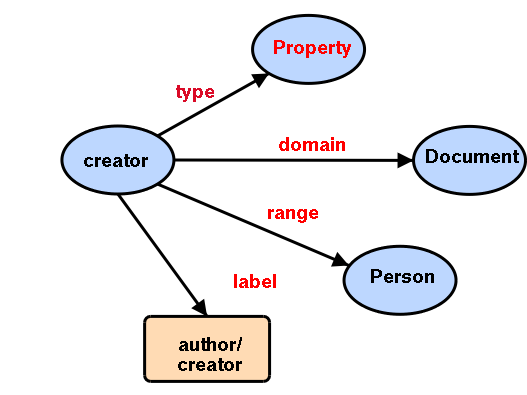
\includegraphics[scale=0.55]{figure2}
%\caption{Popis schémy.}\label{figure2}
%\end{center}\end{figure}
%
%Etiam nec lorem leo, id consequat tellus. Etiam id mattis massa. Phasellus commodo, lacus in viverra lacinia, quam leo ultricies tellus, condimentum vehicula dui nisl a magna. In mi felis, malesuada eget tincidunt eget, rutrum ac lacus. In a nisl tellus. Mauris hendrerit egestas odio ac consequat. Etiam nec lorem leo, id consequat tellus. Etiam id mattis massa. Phasellus commodo, lacus in viverra lacinia, quam leo ultricies tellus, condimentum vehicula dui nisl a magna. In mi felis, malesuada eget tincidunt eget, rutrum ac lacus. In a nisl tellus. Mauris hendrerit egestas odio ac consequat. Etiam nec lorem leo, id consequat tellus. Etiam id mattis massa. Phasellus commodo, lacus in viverra lacinia, quam leo ultricies tellus, condimentum vehicula dui nisl a magna. In mi felis, malesuada eget tincidunt eget, rutrum ac lacus. In a nisl tellus. Mauris hendrerit egestas odio ac consequat.
%
%\lstinputlisting[float=h,language=javascript,caption={Príklad listingu zo súboru.},label={listing},frame=single,frameround=ffff,captionpos=b,basicstyle=\scriptsize]{figures/listing}
%
%Etiam nec lorem leo, id consequat tellus. Etiam id mattis massa. Phasellus commodo, lacus in viverra lacinia, quam leo ultricies tellus, condimentum vehicula dui nisl a magna. In mi felis, malesuada eget tincidunt eget, rutrum ac lacus. In a nisl tellus. Mauris hendrerit egestas odio ac consequat. Etiam nec lorem leo, id consequat tellus. Etiam id mattis massa. Phasellus commodo, lacus in viverra lacinia, quam leo ultricies tellus, condimentum vehicula dui nisl a magna. In mi felis, malesuada eget tincidunt eget, rutrum ac lacus. In a nisl tellus. Mauris hendrerit egestas odio ac consequat. Etiam nec lorem leo, id consequat tellus. Etiam id mattis massa. Phasellus commodo, lacus in viverra lacinia, quam leo ultricies tellus, condimentum vehicula dui nisl a magna. In mi felis, malesuada eget tincidunt eget, rutrum ac lacus. In a nisl tellus. Mauris hendrerit egestas odio ac consequat.
